\documentclass[12pt,a4paper]{report}
\usepackage[T1]{fontenc}
\usepackage[utf8]{inputenc}
\usepackage{charter}
\usepackage{ngerman} \usepackage[left=2cm,right=2cm,top=2cm,bottom=2cm]{geometry}
\usepackage{tikz}
\usepackage{pgfplots}
\usepackage{amsmath}

\begin{document}
	\thispagestyle{empty}
	\paragraph{Einschalten (Magnetisierung):} \mbox{} \\
	Auf Grund des einsetzenden Stromflusses ändert sich $B$ (von Null steigend) und indiziert deswegen direkt eine dem ursächlichen Stromfluss entgegengesetzte Spannung, was somit zur Folge hat, dass der Stromfluss gehemmt wird: \\[1cm]
\vspace{2cm}
	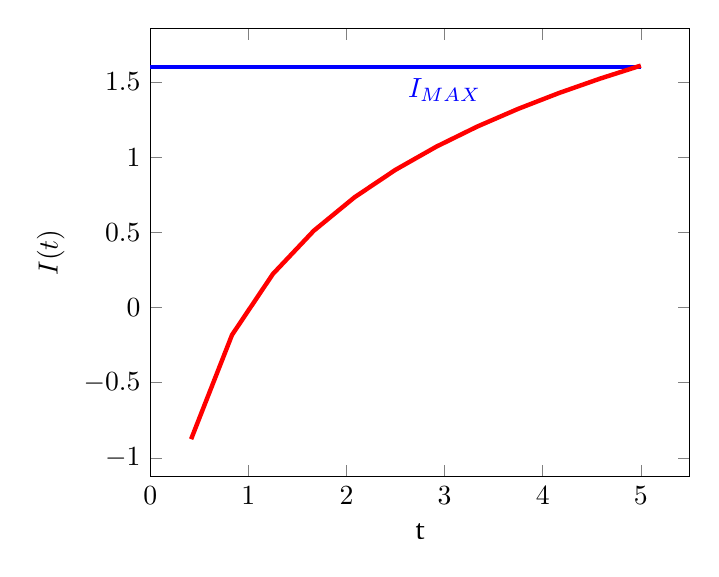
\begin{tikzpicture}
		\begin{axis}[
			xlabel=t,
			ylabel=$I(t)$,
			xmin=0
		]
			\addplot[color=blue,ultra thick]{1.6} node[below, pos=0.8] {$I_{MAX}$};
			\addplot[color=red,ultra thick]{ln(x)};
		\end{axis}
	\end{tikzpicture}
	\vspace{0cm}\\
	\noindent
	Der Strom indiziert somit in der Spule selbst eine Spannung (\textbf{Selbstinduktion}). \\
	$\Rightarrow$ Induktionsgesetz für diesen Fall: \\
	\begin{align*}
		U_{ind} &= -n \cdot \dot \phi(t)\ \ \text{mit}\ \ \phi(t) = A(t) \cdot B(t) \\
		&= -n \cdot A \cdot \dot B(t) \\
		&= -n \cdot A \cdot \mu_0 \cdot \mu_r \cdot \frac{n}{l} \cdot \dot I(t) \\
		&= -\mu_0 \cdot \mu_r \cdot n^2 \cdot \frac{A}{l} \cdot \dot I(t) \\
		L&= \mu_0 \cdot \mu_r \cdot \frac{A}{l} \cdot n^2 \to \text{Induktivität (Magnetisierungsfähigkeit)} \\
		[L] &= 1H = 1\  \text{Henry} \\
		\Rightarrow& U_{ind} = -L \cdot \dot I(t)
	\end{align*}
	Beschreibung der magnetischen Feldstärke \texttt{in} einer Spule:
	\begin{align*}
		B &= \mu_0 \cdot \mu_r \cdot \frac{n}{l} \cdot I(t)
	\end{align*}
	mit\\
	\begin{align*}
		\mu_0&: \text{magnetische Feldkonstante} \\
		&\Rightarrow 4 \cdot \pi \cdot 10^{-7} \frac{V_s}{Am} \\
		n&: \text{Wicklungszahl} \\
		l&: \text{Länge der Spule} \\
		\mu_r&: \text{Permeabilitätszahl (\dq wat is' da für'n Zeug inne Spule\dq)} \\
		&\ \ \ \text{Eisenkern} \approx 5000
	\end{align*}

\end{document}